%!TEX root = ../Thesis.tex
\label{chap:main}

\section{Introduction}
In the first chapter four reseaerch questions were defined, and based on them the experimental design for the pilot study was created. But, given the results of this study and as stated in its discussion, the experimental design for the main study was simplified and therefore the research questions reduced to the following three:\\

\begin{enumerate}[RQ1.-]
        \item In a complex sentence, how does the mood alternation of the embedded verb that occurs due to the negation of the main or matrix verb affect the factuality value of the embedded event?
        \item How does an individual subject affect the factuality judgment of the event?
        \item How does a subject that refers to a collective entity like an institution, affect the factuality judgment of the event?
\end{enumerate}

From these questions we have the already known negation, individual and collective conditions; which can be grouped into specificity conditions (individual and collective) and mood alternation condition (negation). Furthermore, as in the pilot study the negation condition was divide into the categories baseline, indicative, and subjunctive, exemplified in sentences \ref{ex:stmoodaltbas} to \ref{ex:stmoodaltsbjv}. The difference for the specificity conditions is indicated by \textbf{/}.\\

\begin{exe}
  \ex
    \begin{xlist}
      \item  {\gll El presidente/gobierno dijo que el país \textbf{tenía} problemas económicos.\\ the.\M.\Sg{} president.\M.\Sg{} say.\Pst.\Pfv.\Ind.\Tsg{} that the.\M.\Sg{} country.\M.\Sg{} \textbf{have.\Pst.\Ipfv.\Ind.\Tsg{}} problem.\M.\Pl{} economic.\M.\Pl{} \\\ "The president/government said that the country \textbf{had} economic problems."\glt }\label{ex:stmoodaltbas}
      \item  {\gll El presidente/gobierno no dijo que el país \textbf{tenía} problemas económicos.\\ the.\M.\Sg{} president.\M.\Sg{} not say.\Pst.\Pfv.\Ind.\Tsg{} that the.\M.\Sg{} country.\M.\Sg{} \textbf{have.\Pst.\Ipfv.\Ind.\Tsg{}} problem.\M.\Pl{} economic.\M.\Pl{} \\\ "The president/government didn't say that the country \textbf{had} economic problems."\glt }\label{ex:stmoodaltind}
      \item {\gll El presidente/gobierno no dijo que el país \textbf{tuviera} problemas económicos.\\   the.\M.\Sg{} president/government.\M.\Sg{} not say.\Pst.\Pfv.\Ind.\Tsg{} that the.\M.\Sg{} country.\M.\Sg{} \textbf{have.\Pst.\Ipfv.\Sbjv.\Tsg{}} problem.\M.\Pl{} economic.\M.\Pl{} \\\ "The president/government didn't say that the country had economic problems."\glt }\label{ex:stmoodaltsbjv}
    \end{xlist}
\end{exe}

To obtain the experimental design, these conditions were crossed as in the pilot study, obtaining in this case a $3\times2$ design shown in Table \ref{tab:design}, where we also see that the terminology used in the pilot study of seeds and variants is kept here. Although in Section \ref{subsec:pilcompred} it was proved that the veridicality of the matrix verb affects the factuality of the embedded predicate and thus the label chosen by the annotator, it was decided not to include it directly in the experimental design but rather to annotate each pair with this information as it will be explained in the next section and tracked it closely in the analysis of the annotations. This was done to prevent a more complicated experimental design.\\

\begin{table}
\centering
\begin{tabular}{|c|c|c|c|}
\hline
\multicolumn{4}{|c|}{Experimental Conditions}\\\hline
                      & &\multicolumn{2}{c|}{SPECIFICITY} \\\cline{1-4} 
                      & &Individual&Collective\\\cline{2-4} 
\multirow{3}{*}{MOOD-Negation} & Baseline & S1 & S2 \\\cline{2-4}
                      & Indicative & V1 & V2 \\\cline{2-4}
                      & Subjunctive & V1 & V2  \\ \cline{2-4}\hline                                                          
\end{tabular}

\caption[Experimental conditions main study.]{Experimental conditions for the main study. As in the pilot study, \textbf{S} followed by a number stands for set of seeds, \textbf{V} stands for variants, with the number indicating the corresponding set of seeds.}
\label{tab:design}
\end{table}

\section{Dataset}
Different sources were used to create the corpus. First, in order to directly compare results with the pilot study, we used all pairs from the negation condition. Then candidate premises were extracted from a section of the Daves Corpus del Español \citep{daves2016}, the Old News Corpus for Spanish \citep{oldnews}, \textit{El Quijote} by Miguel de Cervantes (as found in \citet{jsdario2017}), the XNLI corpus \citep{conneau2018xnli}, and the United Nations corpus in Spanish for the years 2000, 2001, 2002, and 2003 \citep{eisele2010multiun}. The candidate premises were sentences in the indicative condition whose embedded verbs were not in the simple future or conditional tense and they were found thanks to the LinguaKit \citep{Gamallo95}. After that the following modifications were done:\\
    \begin{itemize}
    \item Premises were shorten to be under 30 tokens, when necessary.
    \item Additional verbs in personal forms were removed.
    \item References were resolved when it was both needed and clear. There was at least one case in which it was needed, but it wasn't clear, and therefore a arbitrary substitution was made.
    \item Collocations like "to be a doubt" were not included.
    \item In a few cases where the verb was in first person (singular or plural) the agent was just put ahead of the premise in the following format: \textit{Lotario: I think that the sky is blue."}
    \item In one case the aspect of the embedded was changed to allow mood alternation since there are no simple forms in perfect aspect for the subjunctive).
    \item Adverbs modifying the matrix verb were removed.
    \item In a few cases, the subject was modified so the premise could be used both for individual and collective conditions.
  \end{itemize}

Once these modifications were done, the hypotheses were extracted and the pairs were modified following the experimental design. Then different lexical, morphological, and statistical labels for each pair were gathered with the idea of maybe using them to extend the analysis of the crowdsourced annotations. The most relevant features gathered are the lexical items corresponding to the matrix and the embedded verbs, the veridicality value of the matrix verb, and person, number, tense and mood for both the matrix and the embedded verb. So for example (\ref{ex:stmoodaltbas} in either of the specificity conditions part of the information we have is the following: \{ matrix: decir, auxiliar: NaN, modal: NaN, veridicality: o/o\footnote{Neutral in affirmative and negative contexts.}, length\_premise: $9$\}\\

It should be noted though that the distribution for most of these labels is quite spreaded and that the veridicality annotations, although done with the help of \citet{stanlex2012}, are my own annotations and they do have a significant degree of uncertainty. Lastly, in order to obtain an overall view of the corpus, counts of these features and some basic statistics were computed. Table \ref{tab:corstats} shows a sample of these.\\


\begin{table}
\centering
\begin{tabular}{|c|c|c|c|}
\hline
\multicolumn{2}{|c|}{Basic Corpus Statistics}\\\hline
                      & Value\\\hline 
\#pairs & $524$ \\\hline
Average premise length &$15.004$\\\hline
Average hypothesis Length & $9.539$\\\hline
\multicolumn{2}{|c|}{Most Frequent Matrices}\\\hline
\textit{saber} (to know)  & $102$\\\hline
\textit{creer} (to believe) & $48$\\\hline
\textit{considerar} (to considerate) & $45$\\\hline
\textit{decir}  (to say) & $36$\\\hline
\textit{anunciar} (to announce) & $36$\\\hline
\end{tabular}
\caption{Some basic corpus statistics.}\label{tab:corstats}
\label{tab:basstats}
\end{table}

\section{Predictions}
\label{sect:pred}
Given that several of the results obtained in the pilot study were unexpected and not completely explained, it was not consider important to define new detailed predictions and thus those from the pilot study, repeated with the needed adaptations in Table \ref{tab:predict}, were kept as guidelines for this experiment, although in this case deviations from them are certainly expected since, as mentioned in the previous chapter we know, for example, that verb matrices affect the factuality of the hypotheses.\\ 

Aside from these label predictions, it is important to remark that, while creating the corpus it was notice that some pairs could be \textit{problematic}, that is, pairs for which disagreement or unexpected labels was considered possible. A deeper explanation of these factors will be given in Section \ref{subsect:man}, so for the moment just mention that some of the factors considerd are the nature of the hypothesis, like \textit{Las mujeres son seres humanos} (women are human beings), indefinite determiners like \textit{algunos} (some), and the type of utterance that the premise is, like assertions vs. questions.\\

\begin{table}
\centering
%\resizebox{0.95\columnwidth}{!}{
\begin{tabular}{|c|c|c|c|c|}
\hline
\multicolumn{5}{|c|}{Label Predictions within Experimental Design}\\\hline
                      & & &\multicolumn{2}{c|}{SPECIFICITY} \\\hline
                      & & & Individual & Collective\\\cline{4-5} 
\multirow{3}{*}{MOOD} & \multirow{3}{*}{Negation} & B & CT+ & CT+ \\\cline{3-5}
                      &                           & I & PR+& PR+ \\\cline{3-5}
                      &                           & S & PS- & PS-\\\hline                                                                           
\end{tabular}
%}
\caption[Label predictions.]{Rough approximation of label predictions for each combination of experimental condition. \textbf{B, I, S} stands for \textit{baseline, indicative, subjunctive}. The only difference from the pilot study is the removal of the no longer used possibility condition and the specificity categories.}
\label{tab:predict}
\end{table}

\section{Procedure}
Annotations were collected on the platform Toloka \citep{Pavlichenko2021crowdspeech} with the same labels as in the pilot study (see Figure \ref{fig:labels}). The interface used was similar to that of the pilot study with the difference being that the labels were ordered from positive (CT+) to not a sentence (NaS). Figures \ref{fig:int} and \ref{fig:intlab} show how it looked like. Workers were paid $\$0.433$ per set of pairs, they were required to be Spanish speakers and were chosen among countries where Spanish is either an official language or one of the most important unofficial ones. Aditionally, after the first sets of annotations were gathered it was decided to choose only top 50\% annotators, and for the final sets, top 30\% annotators. No batches were used since there was no way to ensure annotators did not cross between them, but pairs were gathered in sets of no more than 10, and annotators were allowed to skipped them. As to the number of annotators per pair, we gathered as many as the budget allowed.\\

\begin{figure}
\centering
\parbox{5cm}{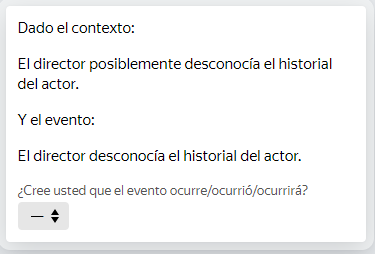
\includegraphics[width=5cm]{final\_study/interface}
\caption{Interface for annotations}\label{fig:int}}
\qquad
\begin{minipage}{5cm}
\includegraphics[width=5cm]{final\_study/interface\_with\_labels}
\caption{Interface with labels}\label{fig:intlab}
\end{minipage}
\end{figure}

While running the experiment, annotations were reviewed with sets of submitted pairs. If the set was submitted too fast, like less than 50 seconds for 10 pairs, or if most of the pairs had the same label (9 out of 10 pairs, for example), it was usually rejected. Control tasks were not added since it was considered that they could lead annotators towards specific labels, or in other words, towards a lexical approach rather than a pragmatic one.\\

Once all annotations were collected, following \citet{pavlick2019inherent} all pairs which were labelled as \textit{not a sentence} by at least one annotator were dropped and if a worker annotated more than 1 pair within a single combination of experimental conditions, all his annotations in that combination were removed. This left a total of 477 pairs and 7 annotators per pair. These are the annotations whose analysis is presented next.\\

\section{Analysis of NaS}
\label{sect:nas}
Before presenting the results of the corpus, I want to briefly see which sentences were excluded due to the use of the label NaS. Although there is previous work on discarding sentences which one annotator considers as not acceptable, given its unexpected use in the pilot study and the decision to change its use, I want to quickly see if there are any underlying patterns that could this rejection. Table \ref{tab:nas} shows some counts of this label.\\ 


\begin{table}
\center
\begin{tabular}{|c|c|c|}
\hline
\multicolumn{2}{|c|}{Use of NaS}\\\hline
                      & Count\\\hline 
Total & $66$\\\hline 
\# pairs & $63$ \\\hline
\# pairs \# NaS $>1$ & $3$\\\hline
\# NaS baseline & $20$\\\hline
\# NaS indicative & $19$\\\hline
\# NaS subjunctive & $24$\\\hline
\# NaS individual & $36$\\\hline
\# NaS collective& $27$\\\hline
\end{tabular}
\caption[Use of NaS]{Basic counts on the use of the label \textit{not a sentence} (NaS).}
\label{tab:nas}
\end{table}

Even though for this experiment there was no explicitly construction whose acceptability I doubted and that the use of this label was explicitly discouraged in the instructions, it was still used in a considerable amount of cases, which suggests that it was a conscious decision. But, as in the pilot study, its use is quite spreaded across the pairs, which questions the exact reason as to why annotators used this label.\\

As to the distribution among experimental conditions, it was expected that the use of NaS would have a similar behaviour as to the disagreement found in the pilot study because it was assumed that non-acceptability is one of the causes of disagreement. But as we can see on the table, this does not seem to be the case. For example, in the pilot study there was more disagreement in the collective condition than in the individual one, but here NaS used more frequently in the individual condition. More importantly, NaS was used quite frequently in the baseline condition, which should not be problematic.\\

In conclusion, not forgetting that the amount of data analyzed here is small and that the analysis itself is shallow, there seems to be no pattern that explains the use of the label \textit{not a sentence} (NaS), thus it appears that there is no support to having this label or to using it as a filter. Next the analysis of the corpus is presented.\\ 

\section{Results}
\subsection{Overview of the Annotations}\label{subsect:overview}
Figure \ref{fig:allbar} shows the distribution of label counts for this experiment. As for the pilot study, the distribution is negatively skewed, but there are also some important differences. First of all, the frequencies for the negative labels are relatively higher than for the previous case. This is probably due to the removal of the possibility condition and the more diversified matrices. Another interesting distintiction relating to the negative labels is the use of the label \textit{certainly not}. In the pilot study negative labels were roughly equally used, at most, the use for CT- was slightly higher, but in this case, the use for this label is lower than the other negative labels. But more important is the situation of the \textit{unknown or uncommited} label, which, contrary to the previous case, is significantly lower than the positive labels. Lastly, it should be noted that here PR+ and PS+ are almost equal, suggesting that the review of one of the annotators of the pilot study (that he couldn't distinguished betwen them) is confirmed.\\

\begin{figure}
\centering
\parbox{10cm}{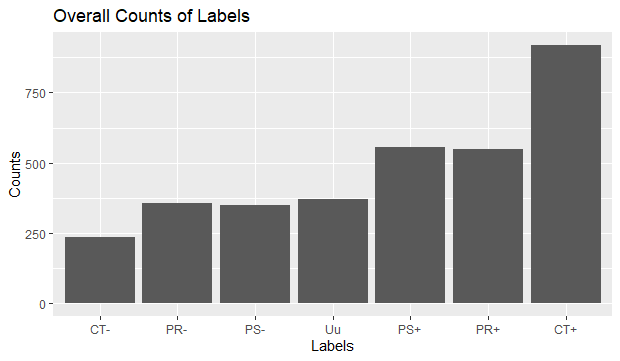
\includegraphics[width=10cm]{final\_study/overallnonas}
\caption{Overall distribution of the proportion of labels used by annotators.}\label{fig:allbar}}
\qquad
\end{figure}

To further understand the overall features of the annotation some very basic computations, shown in Table \ref{tab:basstats}, were done. Regarding the agreement patterns summarized by the counts of pairs with $>3$ votes on one label or majority label, with a unique label but $<3$ votes or most votes label, and without a unique label; they indicate that the inter-annotator agreement score is likely to be quite low, but since for $~80\%$ of the pairs there is 1 label, there might some underlying tendencies that the experiment has not flashed out. Lastly, it should be noted that how spread the number of annotations a worker does is. Next we will go over the inter-annotation agreement scores.\\ 

\begin{table}
\begin{tabular}{|c|c|c|c|}
\hline
\multicolumn{3}{|c|}{Basic Statistics}\\\hline
                      & Count&Percentage\\\hline 
Number of analyzed pairs & $477$ & $88.333$\\\hline
Number of dropped pairs & $63$ & $11.6$\\\hline
Number of analyzed annotations & $3339$ & - \\\hline
Total number of annotators & $248$ & $100$\\\hline
Average annotations per worker & $13.464$ & - \\\hline
Standard deviation annotations per worker & $15.261$ & -\\\hline
Maximum \#annotations per worker & $98$ & - \\\hline
Minimum \#annotations per worker & $1$  & - \\\hline 
\#pairs with $>3$ votes on one label &  $195$ & $41.139$\\\hline
\#pairs with a unique label but $<3$ votes & $201$ & $42.405$ \\\hline                       
\#pairs without a unique label & $78$ & $16.456$\\\hline
\end{tabular}
\caption[Basic counts of the annotations.]{Some basic counts of the annotations.}
\label{tab:basstats}
\end{table}

\subsection{Inter-Annotator Agreement Scores}\label{subsect:iaa}

Overall the inter-annotator agreement score for the whole corpus is $AC_2=0.114$ which is barely within the range of slight agreement $(0.11-0.40)$ \citep{shrout1998measurement} and which is far away from the pilot's study $AC_2=0.388$ for the negation condition. Given this, I decided to explore the value of Gwet's $Ac_2$ for different subsets of the corpus to try to find what causes such big disagreement. Subsetting by veridicality values or by specificity conditions did not yield very informative results, but, as seen in Table \ref{tab:iaa}, subsetting by mood categories or by whether the pair was or not in the pilot gave some interesting results.\\

The biggest difference we see is between the baseline and the mood alternation conditions, there is a drop from fair agreement to virtually none $(0.00-0.10)$, which can be considered as evidence that the baseline is well established. Nevertheless although considerably higher than for the whole corpus, the agreement for the baseline category is still lower than for the pilot study, which at least partially explains why for the other two conditions the score is quite low since mood alternation is a pragmatic phenomen. Furthermore, the difference between the indicative and the subjunctive is minimal, which can be regarded as a sign that mood alternation does not affect the factivity of the embedded event.\\

\begin{table}
\center
\begin{tabular}{|c|c|c|}
\hline
\multicolumn{2}{|c|}{Inter-Annotator Agreement Score for Different Subsets}\\\hline
                     Subset & $AC_2$\\\hline 
ALL & $0.114$\\\hline 
Baseline & $0.194$\\\hline
Indicative & $0.070$ \\\hline
Subjunctive & $ 0.085$\\\hline
Pairs in pilot study & $0.080$ \\\hline
Pairs not in pilot study & $ 0.129$\\\hline
\end{tabular}
\caption[Ac2 subsets.]{Inter-annotator-agreements scores for the whole corpus and different subsets.}
\label{tab:iaa}
\end{table}

A very puzzling result shown on the table is the difference between the pairs that were on the pilot study and those who were not. Since an important difference between the pairs in both studies is that the matrix verbs in the pilot are the standard matrices for mood alternation according to \citet{espanola2010nueva} and those in this study are \textit{natural occurrences}, the corpus was subsetted according to whether the matrix verb is standard or not, but the difference was minimal. Thus the difference between being or not in the pilot study probably does not have a straightforward explanation.\\


\begin{table}
\center
\begin{tabular}{|c|c|c|}
\hline
\multicolumn{2}{|c|}{Inter-Annotator Agreement Score for Different Matrices}\\\hline
                     Subset & $AC_2$\\\hline 
ALL & $0.114$\\\hline 
Top 5 most frequent matrices & $0.123$\\\hline
Not top 5 matrices & $0.093$\\\hline
\textit{saber} (to know) & $0.170$\\\hline
\textit{creer} (to believe) & $0.131$\\\hline
\textit{considerar} (to considerate) & $0.098$\\\hline
\textit{olvidar} (to forget) & $0.181$\\\hline
\textit{ver} (to see) & $0.022$\\\hline
\end{tabular}
\caption[Ac2 matrices.]{Inter-annotator-agreements scores for the whole corpus and different subsets by matrix verb. The 5 most frequent matrices are \textit{saber} (to know), \textit{creer} (to believe), \textit{considerar} (to considerate), \textit{decir} (to say), and \textit{anunciar} (to announce).}
\label{tab:iaamatrix}
\end{table}

Aside from the already metioned subsets, $Ac_2$ was computed on different matrix verbs subsets and the results are presented in Table \ref{tab:iaamatrix}. At first, I suspected that rare matrices could cause disagreement and therefore divided the corpus into two groups: pairs whose matrix verb is one of the 5 most frequent ones (\textit{saber} (to know), \textit{creer} (to believe), \textit{considerar} (to considerate), \textit{decir} (to say), and \textit{anunciar} (to announce)) and the other the rest. This yielded a small difference in the score that I explored even further with specific matrices with different frequencies. By doing so, it was proved that the variations seen with different matrices are not due to the frequency of the matrix but rather to the matrix itself. For example, \textit{saber} (to know) has a frequency of $102$ and an $Ac_2$ score of $0.170$, but, \textit{olvidar} (to forget), whose frequency is $24$, and even of \textit{creer} (to believe, $48$), has an $AC_2$ of $0.181$. In conclusion, it seems that the lexical nature of the matrices influence agreement. Next, I present the results of fitting a cumulative link mixed model (CLMM).\\

\subsection{Model Fitting}\label{subsect:mod}
Several CLMMs with the label as an outcome variable were fitted for both the whole dataset and the datapoints corresponding to the indicative and subjunctive categories. Annotator and premise-hypothesis pair were set as random effects, with the former varely changing within the difference models and the latter showing much greater model variability. As predictors the mood condition, the specificity condition, the different matrix values, and the different veridicality values were used. Predictors were either single or crossed. Maximum number of crossed predictors was 4. AIC values differ, but not greatly: for the whole dataset values were all between $12300$ and $12500$ , with differences smaller than $120$; for the indicative-subjunctive dataset values were between $8300$ and $17500$. Conditional Hessian values range from $10^{2}$ to $10^{5}$.\\

\begin{table}
\center
\begin{tabular}{|c|c|c|c|c|c|c|c|}
\hline
\multicolumn{8}{|c|}{Model Scores}\\\hline
link  &  Threshold & Nobs & logLik & AIC & niter & max.grad & cond.H\\\hline
logit & flexible & $3339$ & $-6179.67$ & $12379.34$ & $964(1997)$ & $7.36\times10^{-03}$ &$1.4\times10^{02}$\\\hline
\end{tabular}
\caption[Model Scores.]{Cumulative link mixed model scores for the model representing the whole dataset.}
\label{tab:modscores}
\end{table}

From these different models there are some important observations than be made. First of all, it seems that the specificity conditions complement other predictors in a few cases, that is, they grade their information rather than being informative on their own. Secondly mood appears to be more relevant than specificity since it can yield significant effects, but when combined with other predictors it seems to grade them or completely disappear. More importantly, for the subset corresponding to the indicative and subjunctive categories there is only one case in which mood has a significant effect: for the matrix verb \textit{olvidar} (to forget). That is, there is a difference between the baseline and the mood alternation conditions, but not between the latter, suggesting that the mood alternation phenomenon in its negation instance does not affect the factuality of the embedded verb significantly. Lastly, given the high conditional Hessian values and the low pair variance reached with the predictors already mentioned, adding more from the information gathered from each pair would be a mistake.\\

\begin{table}
\center
  \begin{tabular}{|c|c|c|c|}
  \hline
  \multicolumn{4}{|c|}{Model Coefficients}\\\hline
  Coefficient & Estimate &Standard Error & Pr($>|z|$)\\\hline
MOOD\_CONDITION: indicative  & $-0.372$ &$0.083$ &$8.32\times 10^{-06}$\\\hline
MOOD\_CONDITION: subjunctive & $-0.438$ &$0.084$ &$1.71\times 10^{-07}$\\\hline 
  \end{tabular}
  \caption[Model Coefficients.]{Cumulative link mixed model coefficients for the model representing the whole dataset.}
  \label{tab:modcoeff} 
\end{table}

To represent the whole dataset, a model with the formula LABEL =  MOOD\_CONDITION + (1 $\mid$ ANNOTATOR) +  (1 $\mid$ ID) was chosen and its main results are presented in tables \ref{tab:modscores} to \ref{tab:modthres}. This model was selected based on the scores presented in Table \ref{tab:modscores} and given that the mood conditions are one of the main variables of this study. Adding the specificity conditions proved to be non-informative and adding the matrices increased both AIC and the conditional Hessian matrix considerably, which was suspected to happen due to their sparse distribution. A similar effect in a lesser degree occurred with the conditional Hessian matrix when adding the veridicality values, and since these values are also quite sparsely distributed, this model was also dismissed.\\  

Table \ref{tab:modcoeff} presents the model coefficients. Both indicative and subjunctive are significantly different from the baseline, thus showing that overall the baseline is well established. Furthermore, both coefficients are negative and rather small, proving the notion expressed in the experiment's predictions on Table \ref{tab:predict}: the factuality of the hypothesis decreases with the negation of the matrix and that overall there is a difference between having the embedded verb in the indicative or in the subjunctive mood. With respect to this difference, it is not so surprising that the models fiited only to the indicative and subjunctive conditions proved insignificant given that the difference between the coefficients in Table \ref{tab:modcoeff} is $<0.1$.\\

\begin{table}
\center
\begin{tabular}{|c|c|c|c|}
\hline
\multicolumn{4}{|c|}{Model Random Effects}\\\hline
Groups  &  Name       &  Variance & Std.Dev.\\\hline
 PAIR  & (Intercept) & $0.101$ &$0.318$\\\hline  
 RATER & (Intercept) & $0.010$ &$0.101$\\\hline  
\end{tabular}
\caption[Model Random Effects.]{Cumulative link mixed model random effects for the model representing the whole dataset.}
\label{tab:modrand}
\end{table}

From Table \ref{tab:modrand}, which presents the random coefficients of the model, the most interesting result is that both random effects are considerably lower than for the pilot study ($0.512$ and $0.505$ respectively). Given the ample disagreement found in this study, one could have expected for it to be reflected in these random variables. In other words, if there was a lot of noise in the data due too a poor collection in the annotations, this would have been meant a lot of variance in the annotator variable. Since this is not true, it seems that the experimental procedure is acceptable and that what should be improved is adding more predictors that could reduce the pair variance. A more balanced corpus could problably solve this.\\ 

\begin{table}
\center
\begin{tabular}{|c|c|c|c|}
\hline
\multicolumn{4}{|c|}{Model Threshold Coefficients}\\\hline
Threshold &  Estimate & Std. Error & z value\\\hline
CT-|PR- &$-2.910$ &$0.089$ &$-32.564$\\\hline
PR-|PS- &$-1.851$ &$0.072$ &$-25.534$\\\hline
PS-|Uu  &$-1.239$ &$0.067$ &$-18.453$\\\hline
Uu|PS+  &$-0.723$ &$0.064$ &$-11.238$\\\hline
PS+|PR+ &$-0.027$ &$0.063$ &$ -0.425$\\\hline
PR+|CT+ &$ 0.724$ &$0.064$ &$ 11.301$\\\hline
\end{tabular}
\caption[Model Threshold Coefficients.]{Cumulative link mixed model threshold coefficients for the model representing the whole dataset.}
\label{tab:modthres}
\end{table}

As to the model threshold coefficients presented in Table \ref{tab:modthres}, we can see that the spaces estimated for each label roughly range from $(0.5-1.2)$, which means that they are closer than in the pilot study, where distances had a rough range of $(0.3-1.5)$. Furthermore, the thresholds here are closer than previously and the differences between negative labels and positive labels have reduced. These three facts together suggest that the label space works better for this corpus than for the previous one.\\

Lastly, in order to understand whether the sparsed distribution of the matrices explains why they do not work well as a predictor, the same model and a model that adds matrix as a predictor were fiited to the subset with the five more frequent matrices where matrix frequencies range from $36$ to $102$. AIC values were almost identical and the model with less predictors had a smaller value for the conditional Hessian matrix. Nevertheless, for the second model the conditional Hessian value was reduced for more than a $100$ and more significant effects (p $<0.05$) were yielded. This confirms what was mentioned above: with a more balanced corpus more predictors than explain the pair variance can be added.\\

Next, an analysis of the different agreement patterns is presented. In other words, an analysis of how votes in each pair are distributed is presented.\\

\subsection{Agreement Patterns}\label{subsect:agrepat}

Given the amount of disagreement found in this study, it seems futile to try to do as in the pilot study and generate a table with the assigned label/s per each combination of experimental combinations. Thus it was decided to instead explore the agreement patterns and see what information they can yield.\\

Figure \ref{fig:pat} shows the distribution of the different agreement patterns found in the corpus. Although there is a considerable amount of patterns that occur less than $25$ times ($<6\%$), there are some patterns which occur with significant frequency which show the lack of agreement meassured by the overall $AC_2$ score. Among these, there are two patterns that more than double the frequencies of the other agreement patterns, $[3,2,1,1]$ and $[2,2,1,1,1]$, and thus they cannot be disregarded.\\

\begin{figure}
%\centering
\parbox{15cm}{\includegraphics[width=15cm]{final\_study/distribution\_of\_agreement\_patterns}
\caption{Distribution of agreement patterns.}\label{fig:pat}}
\qquad
\end{figure}

If we look how the agreement patterns are distributed per mood condition (Figure \ref{fig:moodpat}), we can see that there are some differences, although the picture is not quite clear, and that the results are consistent with the agreement scores in Table \ref{tab:iaa} since within each pattern, pairs are more often in the baseline condition for the patterns that represent greater agremeent and the indicative and the subjunctive more often for the more scattered patterns. Specifically, the baseline condition has the highest frequency from $[6,1]$ to $[3,1,1,1,1]$, and the indicative and the subjunctive are in close competition in patterns from $[2,2,2,1]$ to $[1,1,1,1,1,1,1]$. This suggest that the pairs in the indicative and subjunctive might be better represented with 3 labels, but for the pairs in the baseline condition frequency seem to suggest that 2 label are needed to represent them, which is quite unexpected.\\

\begin{figure}
%\centering
\parbox{15cm}{\includegraphics[width=15cm]{final\_study/agreement\_mood\_conditions}
\caption{Distribution of agreement patterns per mood condition.}\label{fig:moodpat}}
\qquad
\end{figure}

It is quite surprising that there is such a considerable amount of disagreement for pairs that do not have the main linguistic markers in this study, neither negation adverb nor mood alternation. It is true that given this lack of agreement is not surprising that the overall agreement is barely within the range of fair agreement. Given this, it is worthwile to look closer at this condition to try to understand what happened. To do so, we look at all baseline pairs which \textit{negar} as a matrix verb, $6$ in total. Out of these, there is majority agreement for only one pair, three have an agreement of the type most votes, and two do not have an agreement upon unique label. We focus on these last two pairs.\\

Pair (\ref{ex:neg1}) seems to be in the real of uncertainty (PS+ to PS-) since the two most voted labels are PS+ and PS- with two votes each, and there is only one vote for a certainly label, specifically CT+. Having negative labels ($3$ in total) is expected since in positive environments \textit{negar} (to deny) makes the embedded predicated a contradiction. As to why the judgments lean towards uncertainty more than to negative certainty there are two factors that might have some influence: reference solution and the relativity associated with the embedded predicate. Regarding the first factor we have two unresolved references, \textit{su} (his/her) and \textit{esas} (those) that could have caused the workers to wonder whose government and which dispositions is the premise refererring to, and thus made the judgment about the factuality of (\ref{ex:hypneg1}) more uncertain. As to the second factor, \textit{dejar mucho que desear} (to leave much to be desired) is an at least partially subjective expression since what one desires often depends from person to person. Thus when assessing the truthfulness of the hypothesis is likely that the annotators added another layer of uncertainty but, contrary to the previous one, I believe this one depends more on the annotator and more than explaining the uncertainty, it explains the lack of agreement, whereas the layer caused by the reference markers could the most voted labels being PS+ and PS-. But of course, a more thorough analysis is needed to validate this hypothesis.\\

\begin{exe}
  \ex\label{ex:neg1}
    \begin{xlist}
      \item{\gll Su Gobierno niega que la aplicación práctica de esas disposiciones deja mucho que desear.\\ His/her/its.\Sg{} government.\M.\Sg{} deny.\Prs.\Ind.\Tsg{} that the.\F.\Sg{} application.\F.\Sg{} practical.\F.\Sg{} of that.\F.\Pl{} disposition.\F.\Pl{} leave.\Prs.\Ind.\Tsg{} much that desire.\Inf{} \\\glt His/her Government denies that the practical application of those dispositions leaves much to be desired.}
      \item{\gll La aplicación práctica de esas disposiciones deja mucho que desear.\\ the.\F.\Sg{} application.\F.\Sg{} practical.\F.\Sg{} of that.\F.\Pl{} disposition.\F.\Pl{} leave.\Prs.\Ind.\Tsg{} much that desire.\Inf{}\\\glt the practical application of those dispositions leaves much to be desired.} \label{ex:hypneg1}
    \end{xlist}
  \ex\label{ex:neg2}
    \begin{xlist}
      \item{\gll Israel niega que en el ejercicio de su derecho inherente a defenderse del terrorismo más brutal debe actuar dentro de los límites del derecho internacional.\\ Israel deny.\Prs.\Ind.\Tsg{} that in the.\M.\Sg{} exercise.\M.\Sg{} of his/her/its.\Sg{} right.\M.\Sg{} inherent.\Sg{} to defend.\Inf.\Refl{} from.the.\M.\Sg{} terrorism.\M.\Sg{} most brutal.\Sg{} must.\Prs.\Ind.\Tsg{} act.\Inf{} inside of the.\M.\Pl{} limit.\M.\Pl{} of.the.\M.\Pl{} law.\M.\Sg{} international.\M.\Sg{} \\\glt Israel denies that in the exercise of its inherent right to defend itself from the most brutal terrorism must act inside the limits of international law.}
      \item{\gll En el ejercicio de su derecho inherente a defenderse del terrorismo más brutal Israel debe actuar dentro de los límites del derecho internacional.\\ in the.\M.\Sg{} exercise.\M.\Sg{} of his.her.its.\Sg{} right.\M.\Sg{} inherent.\Sg{} to  defend.\Inf.\Refl{} from.the.\M.\Sg{} terrorism.\M.\Sg{} most brutal.\Sg{} Israel must.\Prs.\Ind.\Tsg{} act.\Inf{} inside of the.\M.\Pl{} limit.\M.\Pl{} of.the.\M.\Pl{} law.\M.\Sg{} international.\M.\Sg{} \\\glt In the exercise of its inherent right to defend itself from the most brutal terrorism Israel must act inside the limits of international law.} \label{ex:hypneg2}
    \end{xlist}
\end{exe}

As to pair (\ref{ex:neg2}) the situation is quite different. To begin with we have a 3-way split between PS+, PR+, CT+; which, considering the already mentioned behaviour of \textit{negar} (to deny), is quite surprising. In this case we do not have any unresolved references or subjective predicates, but there is an embedded deontic modal predicate, \textit{debe actuar} (must act), which makes the entire hypothesis an obligation \citep{morante2012modality} and thus making its acceptance or rejection less certain. In other words, the presence of the deontic modal could be the cause of the label split. As to the reason behind most of the labels being in the positive range, it is likely to be the world knowledge associated with the utterance since usually accept the rule of international law, even when having to defend yourself. Consequently overriden the effect of the matrix verb. More examples of how world knowledges affects judgments are presented in the next section.\\

The analysis presented for pairs (\ref{ex:neg1}) and (\ref{ex:neg2}) is obviously not enough to explain the amount of disagreement found in the baseline category, but it provides some evidence that there are other factors that complicate what was supposed to be a \textit{simple} assesment. A more through and formal analysis is left for future work.\\

\begin{figure}
%\centering
\parbox{15cm}{\includegraphics[width=15cm]{final\_study/agreement\_specificity\_conditions}
\caption{Distribution of agreement patterns per mood condition.}\label{fig:specpat}}
\qquad
\end{figure}

Lastly within this section we have Figure \ref{fig:specpat}, which presents the distribution of agreement patterns according to the two specificity conditions: individual and collective. The overall picture appears to be quite confusing with not a very clear sign of for which condition there is more agreement. By distributing the agreement patterns according to their agreement type (majority, most votes, not unique), we see that there are more pairs in the collective condition that have majority agreement, that is, one label with at least 4 votes. But, given that patterns of type most votes (one label has most of the votes but less than 4) are more often in the individual condtion, and that in the pattern with the highest frequency there are clearly more pairs in the collective condition, we cannot confirm the observation made in the pilot study that disagreement was higher for the collective condition. Figure \ref{fig:specpat} rather shows that there are no big differences between the specificity conditions.\\

\subsection{Manual Analysis}
\label{subsect:man}

The goal of this section is to take a closer look at the annotations gathered to search for more causes of disagreement and to see if the \textit{problematic} pairs mentioned in Section \ref{sect:pred} are indeed problematic or not. Before analyzing the pairs it should be noted that to avoid long lists of glossed examples only pairs in the baseline conditions, that is individual or collective seeds, are represented here; that given the results on the specificity conditions not much attention will be payed to them, and more importantly, that this analysis is only exploratory. A systematic analysis is left for future work.\\ 

In the entire corpus no seed was found that \textit{literally} fits the predictions made in Table \ref{tab:predict}, but there are some examples that show small variations between the different mood conditions and a few are close to the predictions. The best example is the pairs represented by seed (\ref{ex:pred1}), which were labelled as CT+, PR+, and PS+, with 4, 3, and 5 votes respectively. The matrix verbs for these pairs, \textit{anunciar} (to announce), is neutral in both affirmative and negative contexts, that is, the premise neither entails nor contradicts the embedded predicate no matter the polarity of the whole sentence. This, together with the absence of any other linguistic markers that could interfer with the mood conditions and that it is unlikely that the hypothesis generates strong presupositions or implicatures, explains the lack of strong deviations from the predictions.\\ 
\begin{exe}
  \ex\label{ex:pred1}
    \begin{xlist}
      \item{\gll La familia anunció que había recortado gastos.\\ the.\F.\Sg{} family.\F.\Sg{} announce.\Pst.\Pfv.\Ind.\Tsg{} that have.\Pst.\Ipfv.\Ind.\Tsg{} cut.down.\Ptcp.\M.\Sg{}expense.\M.\Pl{} \\\glt The family announced that they had cut down expenses.}
      \item{\gll La familia había recortado gastos.\\ the.\F.\Sg{} family.\F.\Sg{} have.\Pst.\Ipfv.\Ind.\Tsg{} cut.down.\Ptcp.\M.\Sg{}expense.\M.\Pl{} \\\glt The family had cut down expenses.} \label{ex:hyppred1}
    \end{xlist}
\end{exe}

Regarding the label assigned for the subjunctive condition is interesting because it suggest that the effect of the negation adverb is not very strong, less than expected. Although a more thourough analysis to fully understand if indeed the impact of \textit{no} (not) in this context.\\

A very interested example is (\ref{ex:mujeres}), for which the label CT+ was assigned in each of the conditions with more than 3 votes, more specifically with 4, 6, and 6 votes respectively. That is, on average the factuality of the event \textit{las mujeres son seres humanos} (women are human beings) is not modified neither by the negation of the matrix verb nor by the mood alternation of the event itself. It is true that this could be explained by the fact that \textit{saber} (to know) implies the embedded predicate in both affirmative and negative contexts, but given that not all pairs that have this matrix verb have these labels, it is likely that the deciding factor is the knowledge associated to the hypothesis. The event represented in the hypothesis is a state whose negation or even just uncertainty is not likely to be accepted in many societies nowadays. In other words, it is likely that the world knowledge of (many of) the speakers overrode all linguistic factors at play.\\

\begin{exe}
  \ex\label{ex:mujeres}
    \begin{xlist}
      \item{\gll Algunos delegados gubernamentales saben que también las mujeres son seres humanos.\\ some.\M.\Pl{} representative.\M.\Pl{} governmental.\M.\Pl{} know.\Prs.\Ind.\Tsg{} that also the.\F.\Pl{} woman.\F.\Pl{} be.\Prs.\Ind.\Tpl{} being.\M.\Pl{} human.\M.\Pl{} \\\glt Some governmental representatives know that women are also human beings.}
      \item{\gll Las mujeres son seres humanos.\\ the.\F.\Pl{} woman.\F.\Pl{} be.\Prs.\Ind.\Tpl{} being.\M.\Pl{} human.\M.\Pl{} \\\glt Women are human beings.} \label{ex:hypmujeres}
    \end{xlist}
\end{exe}

Another good example of how world knowledge affects the factuality judgments is pair (\ref{ex:sex}). In the baseline and indicative conditions this seed received a majority vote for CT+ with 4 votes in each case, and votes for the subjunctive condition were split between PR- and CT+ with 2 votes each. Aside from being in the collective condition and in the respective mood conditions, we have on one hand \textit{negar} (deny), which contradicts the embedded predicate if it is not negated, as a matrix verb, and on the other hand we have \textit{poder} (can), which puts both \textit{negar} and the embedded predicate in the realm of possibilities. Nevertheless, it seems that for most of the annotators neither of these factors were significant, instead I suspect that their world knowledge overrode them since \textit{los jóvenes tienen relaciones sexuales} (young adults have sexual relationships) is often considered an undeniable fact. However, it appears this \textit{universal truth} is not shared by most of the annotators since the same number of annotators that consider the hypothesis as an undeniable fact in the subjunctive condition labelled it as \textit{probably not}. That is, world knowledge can override linguistic features but it is difficult to determine when it is going to happen.\\

\begin{exe}
  \ex\label{ex:sex}
    \begin{xlist}
      \item{\gll Los gobiernos pueden negar que los jóvenes tienen relaciones sexuales.\\ the.\M.\Pl{} government.\M.\Pl{} can.\Prs.\Ind.\Tpl{} deny.\Inf{} that the.\M.\Pl{} young.adult.\M.\Pl{} have.\Prs.\Ind.\Tpl{} relationship.\F.\Pl{} sexual.\Pl{} \\\glt The governments can deny that young adults have sexual relationships.}
      \item{\gll Los jóvenes tienen relaciones sexuales.\\ the.\M.\Pl{} young.adult.\M.\Pl{} have.\Prs.\Ind.\Tpl{} relationship.\F.\Pl{} sexual.\Pl{} \\\glt Young adults have sexual relationships.} \label{ex:hypsex}
    \end{xlist}
\end{exe}

In Section \ref{sect:pred} it was mentioned that some of the pairs in the corpus were questions. Specificially, two seeds were added in the individual condition with certain concern. This concern came because it was assumed that questions would add another level of uncertainty to an already uncertain ground. Thus we will now see what the annotations for these pairs are.\\ 

The seeds for these questions are presented in examples (\ref{ex:q1}) and (\ref{ex:q2}). Both pairs are quite similar since they have the same matrix verb \textit{saber} (to know) in the same tense and aspect, the embedded events are states of different nature but in the same tense, and they even have the same adverb \textit{acaso} (by any chance) modifying the matrix verb. But what is more intersting is that, with the exception of (\ref{ex:q1}) in the subjunctive condition, neither of the variants agree upon one label, although the number of slipts and the labels in which they split are different.\\

\begin{exe}
  \ex\label{ex:q1}
    \begin{xlist}
      \item{\gll ¿Acaso sabe el Sr. Bustani que Israel está armado hasta los dientes con armas nucleares y con las aeronaves y los tanques más avanzados?\\ by.any.chance know.\Prs.\Ind.\Tsg{} the.\M.\Sg{} Mr. Bustani that Israel be.\Prs.\Ind.\Tsg{} arm.\Ptcp{} to the.\M.\Pl{} tooth.\M.\Pl{} with weapon.\F.\Sg{} nuclear.\Pl{} and with the.\F.\Pl{} aircraft.\F.\Pl{} and the.\M.\Pl{} tank.\M.\Pl{} more advance.\Ptcp.\M.\Pl{} \\\glt Does Mr. Bustani know, by any chance, that Israel is armed to the teeth with nuclear weapons and with the more advanced aircrafts and tanks?}
      \item{\gll Israel está armado hasta los dientes con armas nucleares y con las aeronaves y los tanques más avanzados.\\ Israel be.\Prs.\Ind.\Tsg{} arm.\Ptcp{} to the.\M.\Pl{} tooth.\M.\Pl{} with weapon.\F.\Sg{} nuclear.\Pl{} and with the.\F.\Pl{} aircraft.\F.\Pl{} and the.\M.\Pl{} tank.\M.\Pl{} more advance.\Ptcp.\M.\Pl{}\\\glt Israel is armed to the teeth with nuclear weapons and with the more advanced aircrafts and tanks.} \label{ex:hypq1}
    \end{xlist}
    \ex\label{ex:q2}
    \begin{xlist}
      \item{\gll ¿Acaso sabemos todos que cada persona es un microcosmos?\\ by.any.chance know.\F.\Sg{} everyone that each.\F.\Sg{} person\F.\Sg{} be.\Prs.\Ind.\Tsg{} a.\M.\Sg{} microcosmos.\M.\Sg{} \\\glt Do we all know, by any chance, that each person is a microcosmos?}
      \item{\gll Cada persona es un microcosmos\\ each.\F.\Sg{} person\F.\Sg{} be.\Prs.\Ind.\Tsg{} a.\M.\Sg{} microcosmos.\M.\Sg{} \\\glt Each person is a microcosmos.} \label{ex:hypq2}
    \end{xlist}
\end{exe}

In the baseline condition (\ref{ex:q1}) was splitted into PS+/PR+ and (\ref{ex:q2}) into PR-/Uu/CT+, in both cases with 2 votes per label. Given the already mentioned confusion between probability and possibility, the split in the first case is not surprising; and if to that we add the uncertainty assumed for these questions, the chosen labels are both acceptable and explainable. As to the second case is definitely unexpected, but when looking directly at the hypothesis (\ref{ex:hypq2}), it seems that it might be cause of the disagreement. \textit{Cada persona es un microcosmos} (each person is a microcosmos) is a statement of a phylosophical nature, thus some people consider it an \textit{undenniable} truth while others might negate its factuality. Either way, I hypothesize that this kind of events generate strong presuppositions that are more likely to override linguistic markers than other types of events.\\

As to the results for the other two conditions of the seed (\ref{ex:q2}), the explanation holds since the range of labels used is the same, although the splits change. Regarding the variations for (\ref{ex:q1}), there is more variation. In the indicative condition we have again a 2-2 split, but instead we have the labels Uu and CT+. For the subjunctive condition there are no splits at all, instead we have a majority agreement for CT+. The only reasonable explanation appears to be that there is a \textit{struggle} between the linguistic markers and workers' knowledge about the truthfulness of \textit{Israel está armado hasta los dientes con armas nucleares y con las aeronaves y los tanques más avanzados.} (Israel is armed to the teeth with nuclear weapons and with the more advanced aircrafts and tanks.), and in the subjunctive condition annotators favoured the factuality of this hypothesis, which I know to be considered an undenniable truth by some, over the linguistic markers, similar to the results for (\ref{ex:sex}).\\

Regarding the pairs with indefinite determiners, specifically with \textit{algunos} (some), there were no clear patterns found overall. If they cause uncertainty, it seems that it is in a lesser degree in comparison with questions, since only 2 pairs out of 12 had splitted labels. It is true that only 3 pairs reached a majority agreement, but the labels do not reflect a clear lack of confidence in the judgments, specially with the results already explained for seed (\ref{ex:mujeres}).\\

The last factor that could be considered a cause of disagreement was the presence of a modal verb. Initially this was thought mainly for modals modifying the matrices, but after seeing the results for pair (\ref{ex:neg2}), it was decided to examine the pairs where there is a modal verb in the embedded predicate. There are 30 pairs of this type and for half of them there is not unique label upon which annotators agreed on, a percentage quite higher than the overall $16.456\%$. Furthermore, $4$ out of these $15$ pairs were splitted into threee labels. Thus, it appears that the presence of a deontic modal like \textit{deber} (must) causes disagreement. But of course a more thorough analysis is needed to confirm this hypothesis.\\

